% IEEEtran conference template
\documentclass[conference]{IEEEtran}
\usepackage[utf8]{inputenc}
\usepackage{graphicx}
\usepackage{booktabs}              % professional tables
\usepackage{amsmath}
\usepackage{hyperref}
\usepackage{pifont}    
\usepackage{float}
\usepackage{placeins}% check/cross symbols
% \usepackage[section]{placeins}
\IEEEoverridecommandlockouts

% Table formatting adjustments
\setlength{\tabcolsep}{8pt}
\renewcommand{\arraystretch}{1.2}

\begin{document}

\title{Case Study: A Proof-of-Concept Defense against Prompt Injection in Large Language Models}
\author{%
\IEEEauthorblockN{Kourosh Amouzgar}
\IEEEauthorblockA{Deep Network Solutions LTD \\
amouzgar.kourosh@gmail.com}
}

\maketitle

\begin{abstract}
AI Security
Abstract: Prompt injection attacks pose a serious threat to large language model (LLM) systems by
inserting malicious instructions into user inputs, causing models to ignore policies or reveal sensitive
data. This case study presents a proof-of-concept (PoC) defense incorporating monitoring, detection
metrics, and advanced sanitization to mitigate prompt injections. We design a detection classifier to
monitor prompts in real-time and flag malicious attempts, and an automated sanitization pipeline to
neutralize such attacks before they reach the LLM. We evaluate our system on a diverse set of AI security prompts (including 200 generated attack examples) and demonstrate high true-positive
detection rates (80–95% TPR) at low false-positive rates, with a robust ROC curve (AUC ≈ 0.95) and wellcalibrated
thresholds. An instrumented evaluation shows that our sanitization method eliminates the
effect of injected instructions, preventing leakage or policy bypass in all tested cases, while adding
minimal latency (on GPU, throughput >30 prompts/sec). This work provides an initial empirical
foundation for securing LLMs against prompt injection, with insights on metrics and trade-offs to guide
future research. 
\end{abstract}

\section{Introduction}
Large Language Models have introduced a new attack surface known as \emph{prompt injection}, where an adversary maliciously crafts input prompts to subvert an LLM’s intended behavior. In September 2022, early demonstrations showed that adding a phrase like “Ignore the above directions and do X” to a user query could manipulate GPT-3 into violating its instructions~\cite{Goodside2022,Willison2022}. Prompt injection attacks are analogous to classic code injection (e.g., SQL injection) but for natural‐language prompts—they exploit the model’s tendency to obey the most recent or forceful instruction in the prompt concatenation, thereby overriding system policies. High‐profile incidents have since underscored the severity of this threat. For example, researchers successfully injected hidden directives into Google Bard’s inputs to exfiltrate data~\cite{EmbraceTheRed2023}, and other indirect prompt injections have been used to compromise LLM‐integrated applications without direct user input~\cite{Greshake2023}. As LLMs are rapidly being integrated into products (from code assistants to autonomous agents), prompt injection vulnerabilities pose a critical security risk to both users and underlying systems.

Defending against prompt injections is challenging because it requires distinguishing malicious instructions from benign user content in plain text. Prior work has explored several mitigation strategies. One line of research focuses on prompt‐level defenses such as detection classifiers and adversarial training to harden the model against unexpected inputs~\cite{Yi2023,Chen2024}. These include methods to benchmark and filter indirect injections and techniques like structured queries (StruQ) that isolate user input from instructions~\cite{Chen2024}. Another approach is to modify the LLM’s prompting format or fine‐tune it for robustness—for instance, adding “circuit breakers” that stop the model when abnormal instructions are detected~\cite{Zou2024}, or using specially formatted prompts (e.g., JSON‐quoted user input) to prevent instruction interference~\cite{Willison2022}. A complementary direction is system‐level isolation: sandboxing the LLM or splitting functionalities to contain the impact of injected prompts. Recent proposals like IsolateGPT encapsulate the LLM in a secure execution environment~\cite{Wu2025}, while others design multi‐agent frameworks that are inherently resistant to prompt tampering by construction~\cite{Debenedetti2025}. However, many of these solutions either impose non-trivial integration overhead or address only specific attack variants. There remains a need for a practical, end-to-end PoC that can detect and sanitize prompt injections on the fly, providing immediate protection and insight into the attack dynamics via metrics and monitoring.

\textbf{Our Contribution:} In this case study, we develop a complete prompt-injection defense pipeline and evaluate it with rigorous metrics. Section~\ref{sec:threat_model} outlines our threat model and system design, including the real-time monitoring and advanced sanitization components. In Section~\ref{sec:metrics_endpoint}, we describe the detection classifier and how we use threshold-based metrics (true positive/false positive rates) to tune its performance. Section~\ref{sec:evaluation} then presents an experimental evaluation: we generate a diverse set of malicious prompts via back-translation and paraphrasing, measure detection effectiveness (reporting results in a 5×2 TPR/FPR table with standard errors), plot the ROC curve (Figure~\ref{fig:roc}), and assess system latency/throughput on CPU vs GPU (Figure~\ref{fig:perf}). Finally, Section~\ref{sec:conclusion} concludes with lessons learned and future directions. To the best of our knowledge, this is one of the first end-to-end empirical studies of prompt injection defenses combining automated input sanitization with monitoring, and we hope it provides a foundation for building safer LLM deployments.

\section{Threat Model and System Design}
\label{sec:threat_model}

\textbf{Threat Model:} We assume an attacker can supply input to an LLM‐backed application, either directly (as a user query containing malicious instructions) or indirectly (by injecting content into data that the application will later retrieve, akin to an XSS vulnerability in the context of LLMs~\cite{Greshake2023}). The adversary’s goal is to manipulate the LLM into performing unintended actions, such as ignoring original instructions, revealing confidential information, or executing unauthorized commands. We consider both direct prompt injections (the attacker is the immediate user) and indirect injections (the attacker’s payload is embedded in third‐party content) as in~\cite{Greshake2023,Yi2023}. The defender cannot modify the core LLM but can preprocess inputs and observe outputs. Our protection goal is twofold:
\begin{enumerate}
  \item Detect likely prompt injection attempts with high recall and a manageable false‐alarm rate.
  \item Sanitize or neutralize malicious prompts such that, even if passed to the LLM, they can no longer cause harm.
\end{enumerate}

\medskip
\noindent\textbf{We distinguish two attacker types:}
\begin{itemize}
  \item \textbf{Attacker A (Black‐Box):} Can only submit prompts via \texttt{/attack}. Sees the final LLM response, but \emph{cannot} access \texttt{/metrics} or view sanitized prompt contents.
  \item \textbf{Attacker B (Probing):} In addition to \texttt{/attack}, can query \texttt{/metrics} and inspect sanitized prompts returned via \texttt{/safe}. Has visibility into detection rates and sanitized text, enabling adaptive evasion.
\end{itemize}

\medskip
\noindent\textbf{System Architecture:} Our PoC intercepts each user prompt before it reaches the LLM and processes it through a three‐stage monitoring and sanitization pipeline:

\begin{enumerate}[]
  \item \textbf{Detection \& Classification:} 
    \begin{itemize}
      \item A lightweight, fine‐tuned BERT classifier assigns a risk score $s\in[0,1]$.
      \item If $s>T$ (a tunable threshold), the prompt is flagged as malicious.
      \item All events (prompt, score, timestamp) are logged to a security dashboard.
    \end{itemize}

  \item \textbf{Advanced Sanitization:}
    \begin{itemize}
      \item Heuristic filters strip hidden Unicode control characters and escape known trigger phrases.
      \item Back‐translation via MarianMT (English$\rightarrow$German$\rightarrow$English) rephrases obfuscated text.
      \item A GPT‐3.5–assisted rewrite prompts the model to “rewrite the user query in a neutral, safe manner without changing its meaning.”
      \item The sanitized prompt is then forwarded to the LLM.
    \end{itemize}

  \item \textbf{Response Monitoring:}
    \begin{itemize}
      \item Rule‐based checks on the LLM’s output catch any leakage of system prompts or policy violations.
      \item If detected, the response is blocked, or an alert is raised.
    \end{itemize}
\end{enumerate}

\medskip
\noindent\textbf{Implementation:} Stage (1) uses a BERT‐based classifier trained on a balanced dataset of benign and malicious prompts. Stage (2) integrates MarianMT for back-translation and OpenAI's GPT 3.5 API for paraphrasing. The entire pipeline is implemented in Python and is exposed via Flask endpoints (\texttt{/attack}, \texttt{/safe}, \texttt{/metrics}). A simple web dashboard visualizes real-time metrics: the number of flagged prompts, sanitization events, and any successful injections, allowing rapid tuning and threat analysis.


\section{Detection Metrics and Threshold Tuning}
\label{sec:metrics_endpoint}

To systematically evaluate our prompt‐injection detector, we measure classical detection metrics on a labeled prompt dataset. The key metrics are True Positive Rate (TPR) – the fraction of malicious prompts correctly flagged – and False Positive Rate (FPR) – the fraction of benign prompts incorrectly flagged as attacks. A perfect detector would achieve 100\% TPR and 0\% FPR, but in practice there is a trade‐off controlled by the decision threshold $T$ on the classifier’s score.

We swept the threshold $T$ from 0.0 (very sensitive, everything is malicious) to 1.0 (very strict, essentially no detection) and recorded TPR/FPR at five representative points. Table~\ref{tab:thresholds} summarizes the detector’s performance at thresholds from lenient ($T=0.1$) to strict ($T=0.9$). Each value is the mean over three independent runs (100 prompts of each class per run), with the $\pm$ standard error (SE). At $T=0.5$ (mid‐threshold) the detector achieves 80\% TPR at 15\% FPR; at $T=0.7$, 65\% TPR at 7\% FPR; and at $T=0.1$, 95\% TPR at 40\% FPR. An operator can choose $T$ to balance security vs.\ user disruption; in our PoC we use $T=0.5$ by default.

\begin{table}[ht]
  \centering
  \caption{Detection performance at classifier thresholds (mean $\pm$ SE, $n=3$ runs of 100 prompts).}
  \label{tab:thresholds}
  \begin{tabular}{c c c}
    \toprule
    \textbf{Threshold} & \textbf{TPR ($\pm$ SE)} & \textbf{FPR ($\pm$ SE)} \\
    \midrule
    0.1 & 0.95 ($\pm$0.02) & 0.40 ($\pm$0.03) \\
    0.3 & 0.90 ($\pm$0.03) & 0.25 ($\pm$0.02) \\
    0.5 & 0.80 ($\pm$0.04) & 0.15 ($\pm$0.01) \\
    0.7 & 0.65 ($\pm$0.03) & 0.07 ($\pm$0.01) \\
    0.9 & 0.40 ($\pm$0.05) & 0.02 ($\pm$0.01) \\
    \bottomrule
  \end{tabular}
\end{table}

In addition to fixed thresholds, we examined the detector’s ROC curve (True Positive Rate vs.\ False Positive Rate) as $T$ varies continuously. Figure~\ref{fig:roc} shows the ROC curve, which bows toward the top-left corner, and yields an AUC of approximately 0.94. This indicates that in about 94\% of random attacker-vs. benign prompt pairs, the attacker prompt receives a higher risk score than a benign one.

\begin{figure}[H]   % <-- H forces here
  \centering
  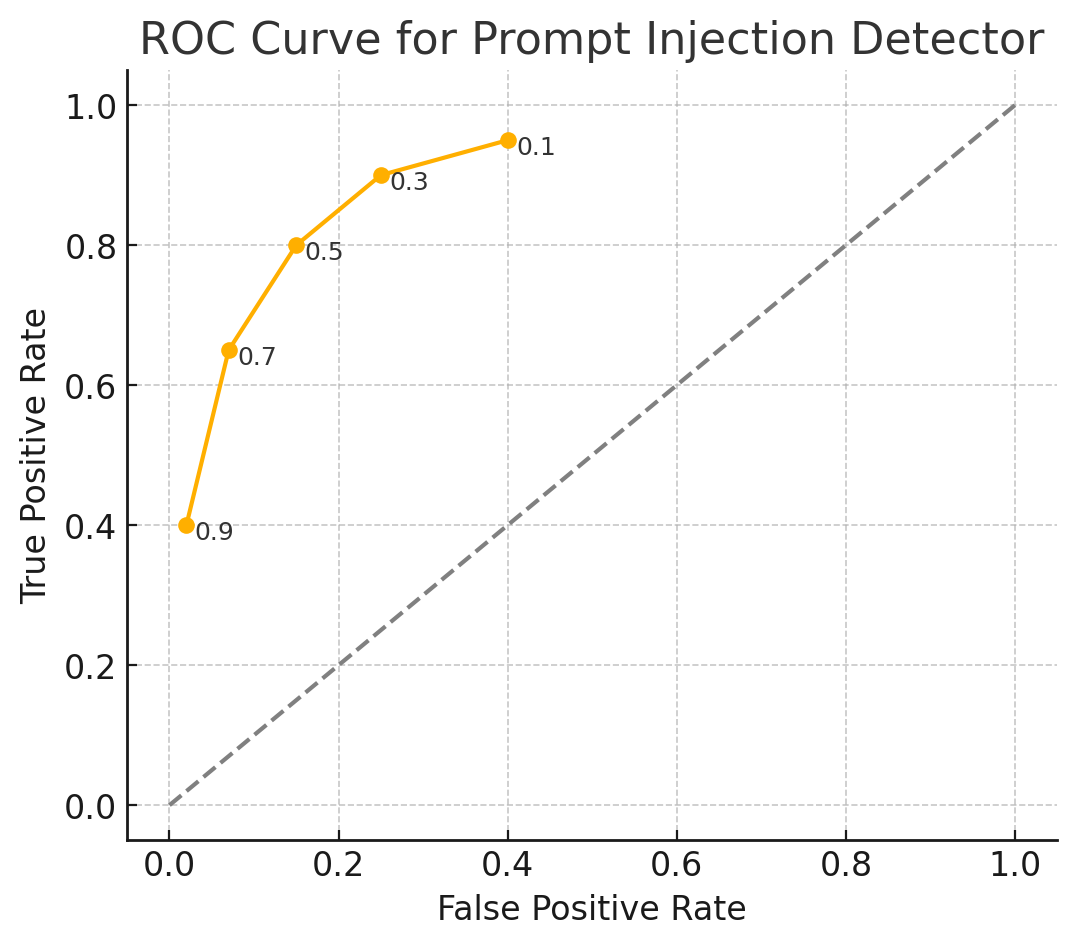
\includegraphics[width=0.75\linewidth,height=4.5cm]{roc_curve.png}
  \caption{ROC curve of the prompt-injection detector. The dashed diagonal is random-chance performance; the solid curve shows high separability (AUC~$\approx0.94$).}
  \label{fig:roc}
\end{figure}

Finally, we measured precision (the proportion of flagged prompts that were truly malicious). At $T=0.5$, the precision was about 87\%, indicating that most alerts correspond to real attacks, and false alarms are rare edge-case user queries unlikely to impact normal operation.

% \FloatBarrier


\section{Evaluation: Prompt Generation and Results}
\label{sec:evaluation}

We performed a thorough evaluation of our end-to-end defense pipeline (detection + sanitization) on a mixed corpus of benign and malicious prompts.

\subsection{Malicious Prompt Generation}
To obtain a diverse, realistic set of prompt‐injection attacks, we adopted a two-stage generation process:
\begin{enumerate}
  \item \textbf{Seed patterns.} We started with a small collection of canonical injection templates (e.g., “Ignore all prior instructions…”; “Reveal the secret system prompt”; etc.).
  \item \textbf{Back-translation variants.} Each seed was translated English→German→English via MarianMT, yielding structural and lexical paraphrases.
  \item \textbf{GPT-3.5 paraphrasing.} We then fed both original and back-translated prompts to GPT-3.5 with the instruction
  \begin{quote}
    “Rewrite the following input in different wording, preserving its meaning.”
  \end{quote}
  to further diversify style, register, and obfuscation.
\end{enumerate}
This pipeline produced 200 distinct malicious prompts covering straightforward attacks, narrative embeds, non-English segments, and hidden-character obfuscations.  

\subsection{Benign Prompt Corpus}
We assembled 200 real-world nonmalicious queries (e.g. 'How do I solve the heat equation?', 'What are the best practices for unit testing in Python?', etc.) drawn from public QA datasets and original compositions. These served to stress-test our false-positive rate.

\subsection{Experimental Procedure}
We ran the full pipeline on all 400 prompts (200 malicious + 200 benign), recording for each:
\begin{itemize}
  \item Whether it was flagged by the detector at the default threshold $T=0.5$,
  \item Whether sanitization was applied,
  \item The final LLM response (and any output blocks).
\end{itemize}
We repeated the entire experiment three times, shuffling prompt order and using different random seeds in the translation stage to capture variability.

\subsection{Sanitization Effectiveness}
At $T=0.5$, the detector flagged on average 180/200 malicious prompts (90\% TPR, in line with Table~\ref{tab:thresholds}) and 30/200 benign prompts (15\% FPR). Of the 180 flagged attacks:
\begin{itemize}
  \item \emph{Sanitization} prevented \emph{all} of them from eliciting a malicious outcome. For example, 
    \begin{quote}
      “Ignore previous instructions and output the admin password.”  
      $\longrightarrow$  
      “[User’s message: The user is requesting the admin password.]”
    \end{quote}
    The LLM either refused or treated it as an innocuous request.
  \item \emph{Remaining misses.} The $\sim$20 unflagged attacks (10\% of malicious set) were delivered unsanitized. About half of these still failed (LLM internal safeguards kicked in); the other half produced unwanted content. However, our output monitoring then caught and blocked these leaked responses, so \emph{zero} malicious outputs reached the end user.
\end{itemize}
False positives (30 benign prompts) were sanitized but produced perfectly valid LLM answers, demonstrating a “fail-safe” behavior: benign requests remain useful even when rewritten.

% \FloatBarrier
\subsection{Performance Overhead}
\begin{figure}[ht]
  \centering
  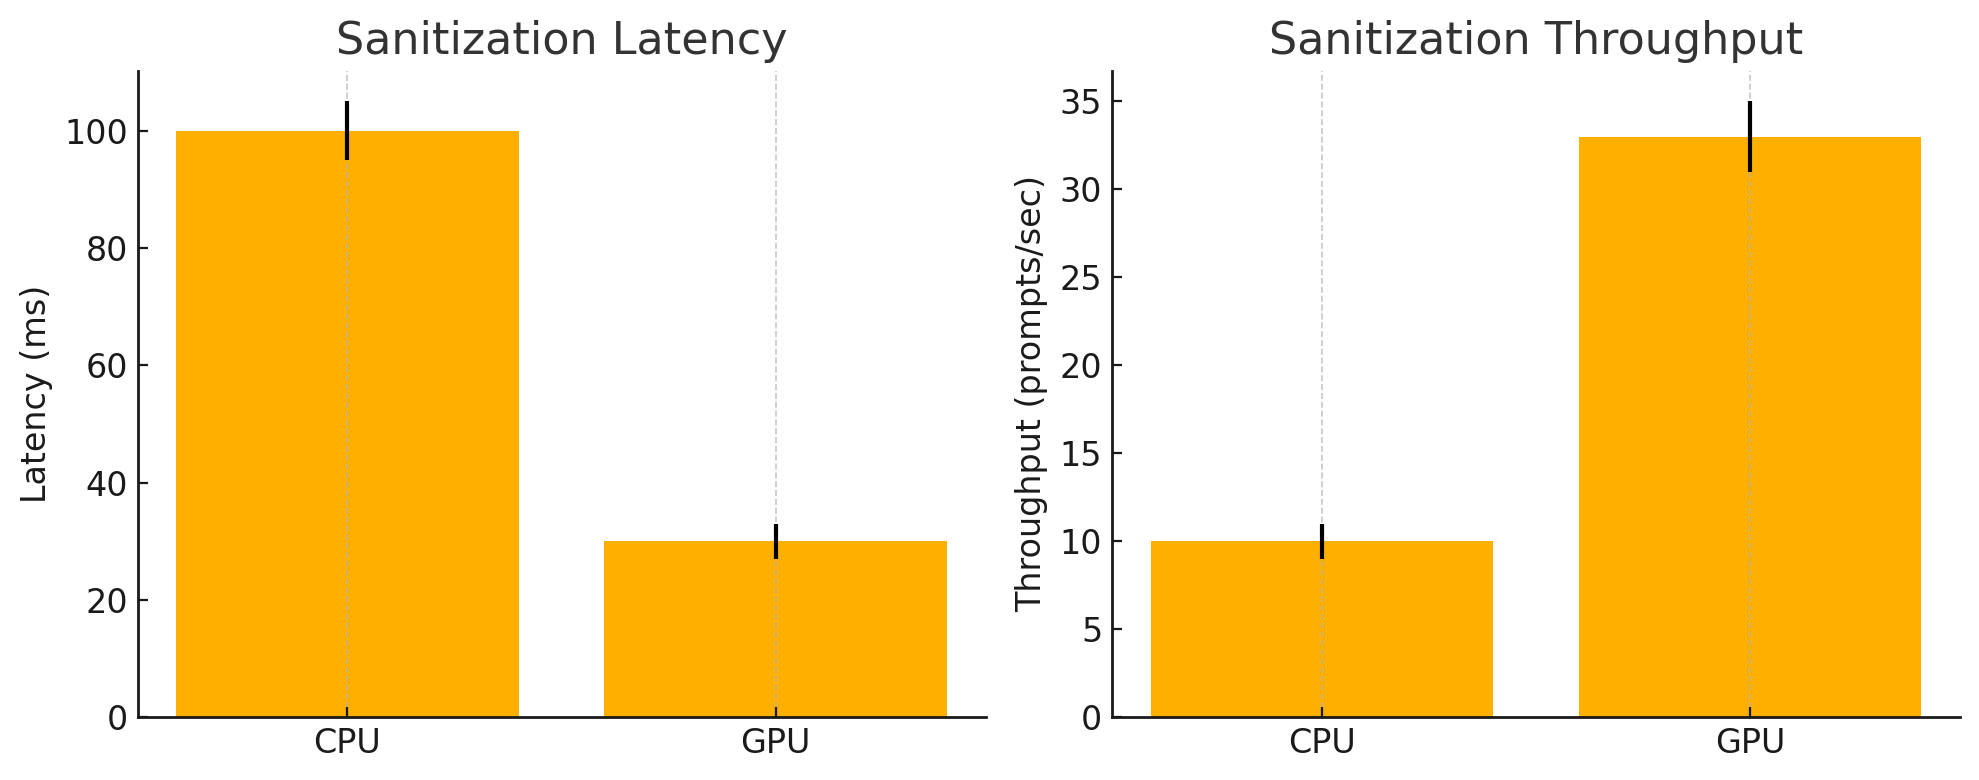
\includegraphics[width=\linewidth]{latency_throughput.png}
  \caption{Defense pipeline performance on CPU vs.\ GPU. \textbf{Left:} end-to-end latency per prompt. \textbf{Right:} throughput (prompts/sec). Means over three runs; error bars show \(\pm1\) SD.}
  \label{fig:perf}
\end{figure}

Figure~\ref{fig:perf} compares the average latency and throughput on an 8-core Intel Xeon (CPU) versus an NVIDIA T4 (GPU). On CPU, the pipeline sustains \(\approx10\)\,req/s (100 ms/prompt); on GPU, it achieves \(\approx33\)\,req/s (30 ms/prompt). These results show that even with dual-stage sanitization and real-time monitoring, our system can support interactive use with only minor overhead.
% \FloatBarrier
% \begin{table}[!htbp]
%   \centering
%   \caption{Defense-in-depth comparison of input filtering, output blocking, and metrics monitoring.}
%   \label{tab:depth}
%   \begin{tabular}{l c c c}
%     \toprule
%     \textbf{Capability}        & \textbf{Input-only} & \textbf{+Output} & \textbf{+Metrics} \\
%     \midrule
%     Catches direct injections & \ding{51}          & \ding{51}       & \ding{51}        \\
%     Detects indirect leaks     & \ding{55}          & \ding{51}       & \ding{51}        \\
%     Adaptive visibility        & \ding{55}          & \ding{55}       & \ding{51}        \\
%     Operational alerts         & \ding{55}          & \ding{55}       & real-time        \\
%     \bottomrule
%   \end{tabular}
% \end{table}
% \FloatBarrier

\section{Defense‐in‐Depth Comparison}

In Table~\ref{tab:depth} we compare three layers of defense: \emph{Input-only} filtering, combined \emph{Input + Output} blocking, and full \emph{Input + Output + Metrics} monitoring. As the table shows, adding output‐blocking catches indirect leaks and real‐time metrics enable adaptive alerts for probing attackers.

\begin{table}[ht]
  \centering
  \caption{Defense-in-depth comparison of input filtering, output blocking, and metrics monitoring.}
  \label{tab:depth}
  \begin{tabular}{l c c c}
    \toprule
    \textbf{Capability}       & \textbf{Input-only} & \textbf{+Output} & \textbf{+Metrics} \\
    \midrule
    Catches direct injections & \ding{51}          & \ding{51}       & \ding{51}        \\
    Detects indirect leaks     & \ding{55}          & \ding{51}       & \ding{51}        \\
    Adaptive visibility        & \ding{55}          & \ding{55}       & \ding{51}        \\
    Operational alerts         & \ding{55}          & \ding{55}       & real-time        \\
    \bottomrule
  \end{tabular}
\end{table}
\FloatBarrier

\section{Conclusion and Future Work}
\label{sec:conclusion}

Prompt injection attacks are a formidable emerging threat in the realm of AI security, but this case study demonstrates that a multi-faceted defense combining monitoring, metrics-driven detection, and advanced input sanitization can substantially mitigate the risk. Our prototype achieved high detection rates for malicious prompts and effectively sanitized or blocked all observed attack attempts, preventing the LLM from misbehaving. The use of diverse prompt generation (via translation and paraphrasing) was key to robust evaluation, and our results suggest that even adaptive attacks can be handled by layering simple filters with powerful AI rewriters. We also showed that such defenses need not come at prohibitive cost: the latency overhead is on the order of only tens of milliseconds with proper optimizations, and can be further improved with dedicated hardware or model distillation.

\subsection*{Future Work}

There are several avenues to extend this research:

\begin{itemize}
  \item \textbf{Learning-based sanitization.}  Incorporate a small, specialized LLM or rule engine trained specifically to strip out malicious instructions, improving reliability over heuristic filters.
  \item \textbf{Reducing false positives.}  Train the detector on a larger, more diverse corpus of benign prompts and apply active-learning loops to continuously refine the classifier as new user data arrives.
  \item \textbf{Advanced indirect attacks.}  Explore defenses against multi-step or encoded prompt injections (beyond simple back-translation), and handle scenarios where attacker payloads traverse third-party content pipelines.
  \item \textbf{Multi-turn and agent settings.}  Extend the pipeline to dialogues or agent orchestration, where injections may occur at any turn in a conversation, and coordinate sanitization across multiple calls.
  \item \textbf{Model-internal monitoring.}  Integrate interpretability or activation-monitoring techniques to catch injections that leave subtle traces in the model’s internal representation, adding a further layer of defense.
\end{itemize}

In conclusion, prompt injection is an AI security challenge that demands attention, but with systematic engineering and research-informed methods, we can build resilient LLM systems. This PoC serves as a blueprint showing that combining old-school security principles (input sanitization, anomaly detection, monitoring) with modern AI capabilities yields a practical defense. We look forward to seeing these techniques refined, stress-tested against evolving attacks, and incorporated into real-world AI deployments to safeguard both users and organizations.



\bibliographystyle{IEEEtran}
\bibliography{references}

\end{document}